\documentclass[journal]{IEEEtran}
\usepackage{cite}
\usepackage{amsmath,amssymb,amsfonts}
\usepackage{algorithmic}
\usepackage{graphicx}
\usepackage{textcomp}
\usepackage{xcolor}
\usepackage{url}
\usepackage{booktabs}
\usepackage[caption=false]{subfig}
\usepackage{multirow}
\usepackage{CJKutf8}
\usepackage{listings}
\usepackage{algorithm}

% Helper macros for consistent notation
\newcommand{\etal}{\textit{et al.}}
\newcommand{\ie}{\textit{i.e.}}
\newcommand{\eg}{\textit{e.g.}}

\begin{document}

\title{Camerala: A Privacy-Preserving Web Framework for Unobtrusive Longitudinal Context-Aware Monitoring}

\author{Kotaro Furukawa, \IEEEmembership{Student Member, IEEE}
\thanks{Manuscript received March 24, 2026; revised Month Day, 2026. This work was supported by the College of Transdisciplinary Sciences for Innovation, Kanazawa University.}
\thanks{K. Furukawa is with the College of Transdisciplinary Sciences for Innovation, Kanazawa University, Kanazawa, Ishikawa 920-1192, Japan (e-mail: kotaro0530@stu.kanazawa-u.ac.jp).}}

\markboth{IEEE Transactions on Affective Computing,~Vol.~XX, No.~X, Month~2026}%
{Furukawa: Unobtrusive Web-Based Sensing Framework}

\maketitle

% =================================================================================
% ABSTRACT
% =================================================================================
\begin{abstract}
Ubiquitous affective computing faces critical bottlenecks: protecting user privacy in domestic spaces and correctly interpreting physiological signals across shifting contexts. We propose \textbf{Camerala}, a privacy-preserving web sensing framework for unobtrusive longitudinal monitoring. By executing remote photoplethysmography (rPPG) and facial landmark tracking entirely within the browser via WebAssembly, Camerala eliminates raw video transmission, solving the "privacy bottleneck." To evaluate its deployability in the wild, we conducted a 10-session autoethnographic proof-of-concept study comparing physiological reactivity between a University Laboratory and a private Home setting. The system successfully captured "Invariance Breaking": a cognitive stressor induced sympathetic mobilization (freezing, accelerated reaction times) in the Lab, but this autonomic response vanished in the Home. This demonstrates Camerala's robust edge-computing capabilities and highlights the critical necessity of context-aware, environmentally parameterized models for next-generation pervasive affective systems.
\end{abstract}

\begin{IEEEkeywords}
Web-based Sensing, Single-Case Experimental Design, Invariance Breaking, Remote Photoplethysmography (rPPG), 
Affective Computing, Ecological Validity, Context Dependency, Polyvagal Theory, Challenge and Threat, Privacy-Preserving AI.
\end{IEEEkeywords}

% =================================================================================
% SECTION 1: INTRODUCTION
% =================================================================================
\section{Introduction}

\IEEEPARstart{T}{he} vision of Affective Computing, as originally articulated by Picard within the MIT Media Lab in the late 1990s \cite{picard_affective_computing}, 
was to endow machines with the capacity to recognize, interpret, simulate, and potentially influence human emotions. 
For over three decades, this vision has catalyzed extensive interdisciplinary research spanning computer science, psychology, 
neuroscience, and biomedical engineering. The ability to automatically detect user states—ranging from frustration and stress 
to engagement and flow—promises to revolutionize human-computer interaction (HCI), enabling systems that adapt dynamically 
to the user's cognitive and emotional needs.

Early work in this domain was predominantly conducted in highly controlled laboratory environments. 
Researchers utilized medical-grade sensors—such as electrocardiograms (ECG) to measure heart rate variability (HRV), 
electroencephalograms (EEG) to monitor cortical asymmetry, and galvanic skin response (GSR) sensors to track sympathetic arousal. 
These pioneering studies successfully established the somatic markers of basic emotions, enabling the development of classifiers 
that could distinguish high-arousal states (e.g., anger, fear) from low-arousal states (e.g., sadness, relaxation) with remarkable accuracy. 
Indeed, within the sanitized, noise-free confines of a sound-proofed laboratory, with a participant wired to a stationary rig, 
we can predict acute stress with near-perfect fidelity.

However, as the field matures and transitions from the laboratory to "in-the-wild" applications \cite{ambulatory_assessment}, 
a fundamental disconnect has emerged between the capabilities of these models and the complexity of real-world human experience. 
This disconnect, which we term the "Contextual Gap," places the field at a critical juncture: we have successfully democratized 
the \textit{sensors} to measure physiology anywhere (via smartwatches, rings, and now standard webcams), 
but we critically lack the \textit{contextual models} to interpret these signals correctly outside the lab.

\subsection{The Crisis of Contextual Rigidity and "Invariance Breaking"}
Current affective computing systems, particularly those deployed in consumer wearables or smart environments, 
often operate on the implicit assumption of \textit{Physiological Invariance}. 
In machine learning terms, this assumes that the conditional probability of an affective state $Y$ given a physiological signal $X$, denoted as $P(Y|X)$, is stationary across all domains $D$.
However, we argue that this mapping is fundamentally non-stationary and dependent on the environmental context $E$:
\begin{equation}
    P(Y|X, E_{lab}) \neq P(Y|X, E_{home})
\end{equation}
This discrepancy leads to what we define as **"Invariance Breaking"**—the systematic failure of affective models when transferred between environments.
A model trained to detect stress in a driving simulator may completely fail when applied to a user sitting in their living room, 
not because the sensor is broken, but because the underlying causal structure of the physiological response has shifted.
The "stress" response in a laboratory—characterized by vigilance and sympathetic mobilization—may be physiologically distinct from "stress" at home, where safety cues damp the autonomic response.

\subsection{Theoretical Framework: Contextual Reactivity}
To address Invariance Breaking, we ground our design in the Biopsychosocial Model \cite{biopsychosocial_model} and Polyvagal Theory \cite{polyvagal, porges_safe_haven}. 
These frameworks suggest that identical cognitive stressors can elicit fundamentally different physiological responses based on environmental appraisal.
In unfamiliar, evaluative environments (like a University Laboratory), a stressor triggers "Threat" (sympathetic mobilization, vasoconstriction, freezing). 
Conversely, a private, familiar environment (like a Home) acts as a "Safe Haven," engaging the ventral vagal complex to dampen sympathetic reactivity. 
Therefore, robust ubiquitous systems must dynamically parameterize their physiological baseline against the user's context.

\subsection{Research Questions and Contributions}
This paper introduces Camerala and investigates its feasibility for context-aware monitoring through an autoethnographic case study, bridging the gap between advanced psychophysiological theory and modern web engineering.
We pose two primary Research Questions (RQs):
\begin{itemize}
    \item \textbf{RQ1 (Framework Feasibility)}: Can a purely client-side, privacy-preserving web framework (Camerala) be reliably deployed in contrasting real-world environments without requiring specialized hardware?
    \item \textbf{RQ2 (Invariance Breaking Demonstration)}: As a proof-of-concept, can this framework capture the hypothesized context-dependent shifts in physiological reactivity ("Invariance Breaking") between an evaluative Laboratory setting and a private Home setting?
\end{itemize}

To answer these questions, we developed \textbf{Camerala}, a purpose-built framework for longitudinal, context-aware affective experimentation. 
Our contributions are threefold:

\begin{enumerate}
    \item \textbf{Camerala Framework}: We present a robust, open-source architecture for client-side physiological sensing. 
    By processing all video data locally within the browser (Edge Computing), Camerala solves the "Privacy Bottleneck" 
    that hinders longitudinal video collection in private homes. We detail the implementation of rPPG and facial landmark tracking 
    using WebAssembly for real-time performance.
    
    \item \textbf{Autoethnographic Deployment Strategy}: We demonstrate the utility of autoethnographic case studies (via Single-Case Experimental Design) for ubiquitous systems evaluation. While large-N group studies are necessary for broad psychological generalizations, dense longitudinal sampling ($N=1, T=600$) serves as a powerful feasibility stress-test for capturing delicate context-dependencies in real-world scenarios.
    
    \item \textbf{Proof-of-Concept Case Study on Contextual Buffering}: Through a 10-session deployment, we provide a concrete demonstration of "Invariance Breaking." We show that the system successfully detects behavioral and physiological signatures of "Threat" in the Lab, while capturing their attenuation at Home. This highlights the practical necessity for context-aware affective models in future scalable deployments.
\end{enumerate}

The remainder of this paper is organized as follows: Section II reviews the state-of-the-art in remote sensing and context-awareness. 
Section III details the technical implementation of Camerala. Section IV describes our SCED methodology. 
Section V presents detailed statistical results. Section VI discusses the theoretical implications for ubiquitous computing, and Section VII concludes.

% =================================================================================
% SECTION 2: RELATED WORK
% =================================================================================
% =================================================================================
% SECTION 2: RELATED WORK
% =================================================================================
\section{Related Work}

\subsection{Remote Physiological Sensing (rPPG)}
Non-contact physiological measurement has evolved from Blind Source Separation (e.g., ICA \cite{poh_ica}) to Model-Based optics (e.g., POS \cite{wang_pos}), and recently to Deep Learning (e.g., DeepPhys \cite{deepphys}). 
While state-of-the-art CNNs offer high accuracy in controlled settings, they frequently suffer from "Domain Shift" when deployed in-the-wild, severely degrading in unstructured lighting or motion \cite{mcduff_rppg}. 
To ensure cross-context robustness and real-time client-side performance, Camerala adopts a physics-based approach, isolating the pulse signal robustly against rigid head motion.

\subsection{Context-Awareness in Affective Computing}
The concept of "Context" in computing was formalized by Dey (2001) as "any information that can be used to characterize the situation of an entity."
In Affective Computing, however, the integration of context has been slow and superficial.
We categorize existing approaches into three levels of sophistication:

\subsubsection{Level 0: Context-Agnostic}
The majority of commercial "Stress Detection" algorithms fall here. They apply a static threshold: $HR > 90 \to Stress$.
This fails in virtually all real-world scenarios due to the physiological confound of physical activity (metabolic demand vs. psychological stress).

\subsubsection{Level 1: Context-as-Feature}
Modern multimodal systems append context data to the feature vector. For example, a classifier might take inputs $[HR, GSR, Location_{GPS}, Noise_{dB}]$.
The model learns to adjust its decision boundary based on location.
While an improvement, this approach treats context as just another noisy sensor input.
It assumes that the relationship between context and physiology is linear and additive.

\subsubsection{Level 2: Context-as-Moderator (Interactionist)}
Our work advocates for this theoretical level. We argue that context is not a feature; it is a \textit{lens} that fundamentally alters
the semantic meaning of physiological arousal.
Based on the Interactionist Theory of Emotion, emotion is constructed from the collision of Core Affect (Arousal/Valence) and Conceptual Knowledge (Context).
The \textit{same} core affect (high arousal) becomes "Fear" in a dark alley but "Excitement" on a roller coaster.

\subsection{Methodological Shifts: Large-N vs. SCED}
The "Gold Standard" in HCI research has long been the Between-Subjects Randomized Controlled Trial (RCT), typically with $N=20 \sim 30$.
This design assumes that by averaging across many individuals, individual differences will cancel out as "noise," revealing the "true" population effect.
However, in psychophysiology, individual differences are not noise; they are the dominant source of variance.
\begin{enumerate}
    \item \textbf{The Baseline Problem}: Person A's resting HR might be 60 bpm; Person B's might be 90 bpm. Averaging them is meaningless.
    \item \textbf{The Reactivity Problem}: Person A might be a "Vascular Responder" (BP spikes), while Person B is a "Cardiac Responder" (HR spikes).
\end{enumerate}
Pooling these heterogeneous phenotypes often washes out significant effects, leading to Type II errors.
Single-Case Experimental Design (SCED) \cite{barlow_sced} avoids this aggregation fallacy.
By treating the individual as their own control and sampling them repeatedly (in our case, 600 trials),
we achieve high statistical power to detect \textit{idiographic} causal relationships.

\subsection{Privacy-Preserving Edge AI}
A major barrier to longitudinal affective computing is the "Privacy Paradox": users desire personalized services but are increasingly wary of surveillance.
Current commercial solutions (e.g., Affectiva, Amazon Halo) rely on cloud-based inference, streaming raw video or audio to centralized servers.
This architecture poses unacceptable risks for monitoring in intimate spaces like the home (e.g., bedrooms).
\begin{itemize}
    \item \textbf{Cloud Architecture}: High latency, high privacy risk. Raw data leaves the device.
    \item \textbf{Edge Architecture}: Zero latency, zero privacy risk. Raw data is processed locally; only anonymous features (HR, RT) are stored.
\end{itemize}
Recent advances in WebAssembly (Wasm) and WebGPU have made high-performance computer vision possible in the browser.
By compiling C++ libraries (OpenCV, MediaPipe) to Wasm, we can run state-of-the-art inference at native speeds (60 FPS)
without a single byte of video data leaving the user's machine. Camerala leverages this paradigm to resolve the Privacy Paradox,
enabling ethical, long-term monitoring of intimate states.
% =================================================================================
% SECTION 3: SYSTEM ARCHITECTURE
% =================================================================================
\section{System Architecture: Camerala}
\textbf{Camerala} (derived from "Camera" + "Laboratory") is a comprehensive, open-source web framework designed
for high-temporal-resolution physiological experimentation. Unlike traditional cloud-based platforms (e.g., Pavlovia, Gorilla)
that operate on a client-server architecture, Camerala employs a "Thick Client" (Edge Computing) philosophy.
This architectural choice is driven by two critical non-functional requirements: \textbf{Privacy Preservation} and \textbf{Real-Time Latency}.

\begin{figure}[t]
    \centering
    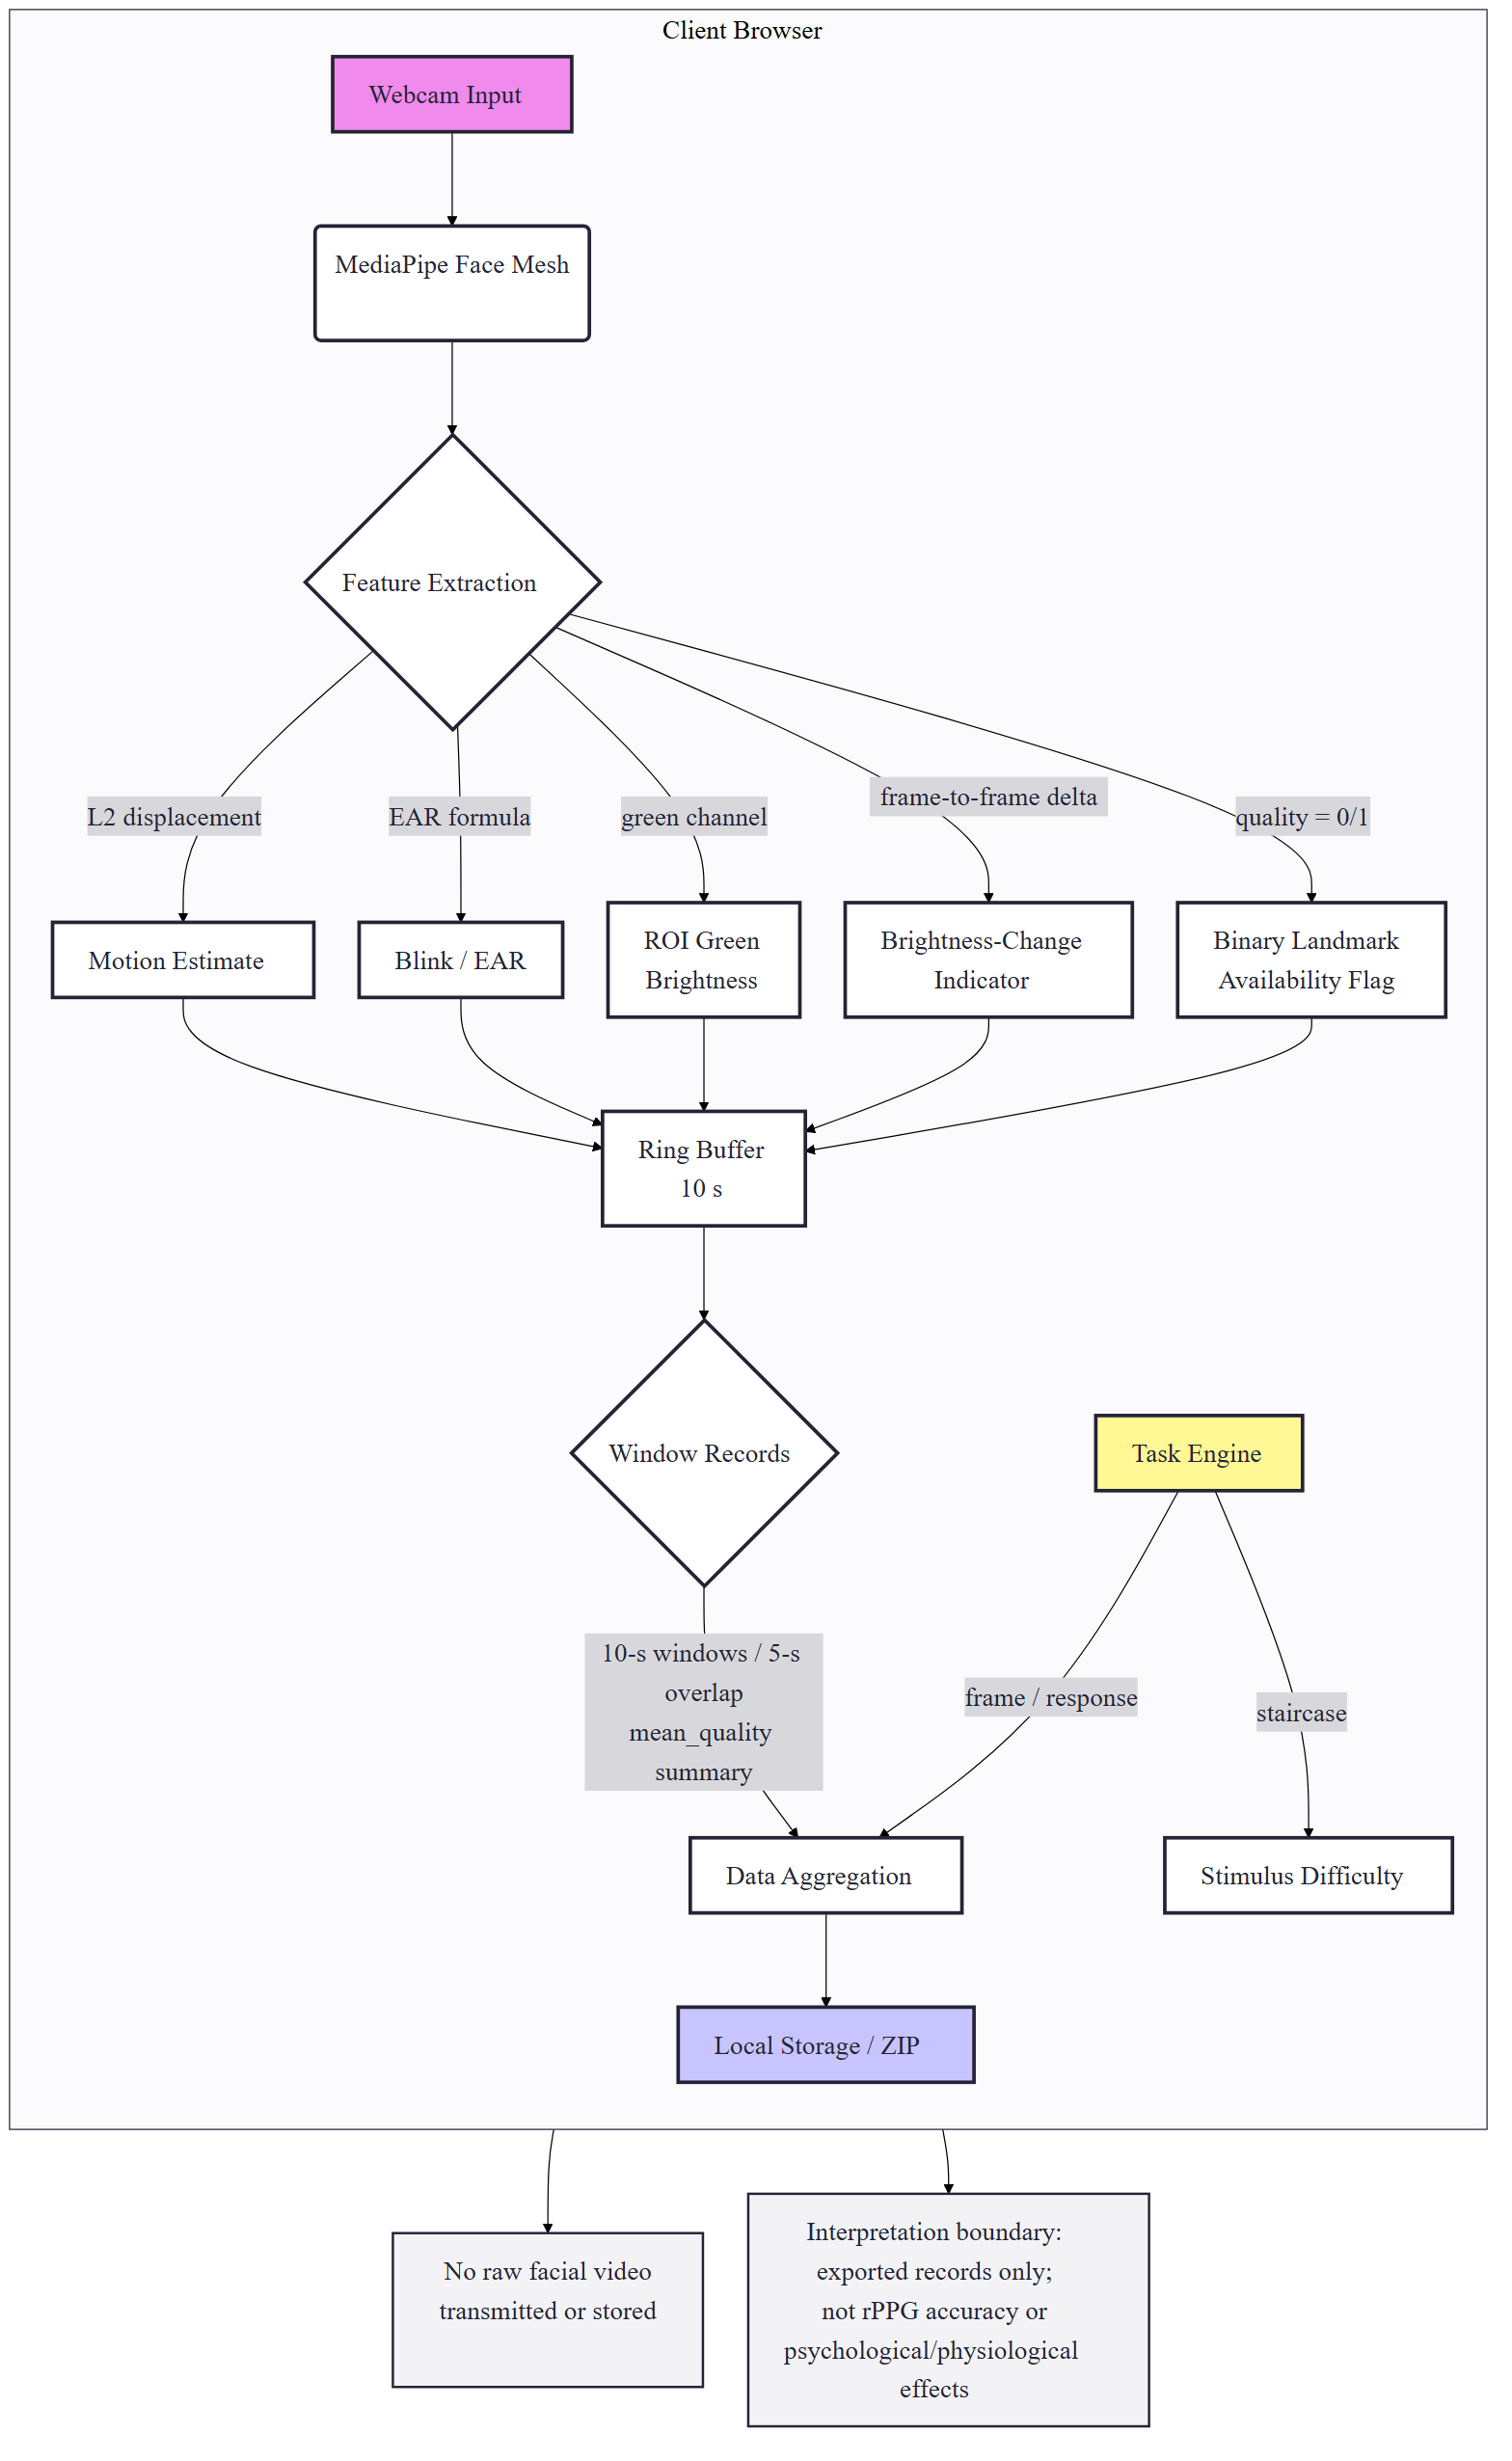
\includegraphics[width=\linewidth]{paper_figures/Figure1_SystemPipeline.png}
    \caption{Overview of the Camerala System Architecture. The system runs entirely client-side, processing webcam frames via MediaPipe Face Mesh (Wasm) to extract rPPG and Head Motion signals in real-time. Data is synchronized with the Psychophysics Task Engine (Canvas API) and stored locally, ensuring no raw video ever leaves the user's device.}
    \label{fig:system_architecture}
\end{figure}

\subsection{High-Level Architecture}
The system enables a complete experimental loop entirely within the browser sandbox (see Fig. \ref{fig:system_architecture}).
The architecture consists of three coupled modules running on the main JavaScript thread and dedicated WebWorkers:
\begin{enumerate}
    \item \textbf{The Task Engine}: Responsible for stimulus rendering, trial logic, and reaction time measurement.
    \item \textbf{The Vision Pipeline}: Responsible for ingesting the webcam stream, performing facial landmark inference, and extracting raw physiological signals.
    \item \textbf{The Data Manager}: Responsible for fusing the asynchronous streams (Vision Frame Time vs. Task Event Time) and securing data persistence.
\end{enumerate}

\subsection{Technical Implementation: The Vision Pipeline}
We utilize the MediaPipe Face Mesh \cite{mediapipe_paper} solution, which provides 468 3D facial landmarks in real-time.
This model is executed via TensorFlow.js with the WebGL backend to leverage the client's GPU acceleration.

\subsubsection{Feature Extraction Logic}
To quantify psychophysiological states, we extract two primary signals: \textit{Head Motion (Freezing)} and \textit{Exposure Fluctuation}.

\textbf{1. Head Motion Index ($M_t$)}
The physiological "Freeze Response" (a defensive reaction to threat) translates to a reduction in gross motor movement.
We capture this by tracking the displacement of rigid cranial landmarks (Nose tip, Left/Right Tragus) that are unaffected by facial expressions.
Let $L_i^t = (x_i^t, y_i^t, z_i^t)$ be the 3D coordinate of the $i$-th landmark at frame $t$.
The instantaneous motion scalar $M_t$ is defined as the Euclidean distance summed over the set of rigid landmarks $S_{rigid} = \{1, 33, 263\}$ (Nose, L-Ear, R-Ear):
\begin{equation}
    M_t = \frac{1}{|S_{rigid}|} \sum_{i \in S_{rigid}} || L_i^t - L_i^{t-1} ||_2
\end{equation}
To ensure scale invariance (handling users sitting at different distances), the coordinates are normalized by the Inter-Ocular Distance (IOD),
calculated as the Euclidean distance between the lateral canthi of the eyes.

\textbf{2. Exposure Fluctuation ($E_{fluc}$)}
Ecological validity introduces noise. In a home environment, lighting is uncontrolled.
Clouds passing the sun, screens flickering, or 60Hz power cycles induce luminance changes that can mask the rPPG signal.
Instead of filtering this out, we quantify it as an independent variable to represent "Contextual Noise."
We define a Region of Interest (ROI) on the forehead, $R_{fore}$. The average luminance $Y_t$ is computed from the RGB channels:
\begin{equation}
    Y_t = \frac{1}{N_{px}} \sum_{(u,v) \in R_{fore}} (0.299R_{u,v} + 0.587G_{u,v} + 0.114B_{u,v})
\end{equation}
The Exposure Fluctuation metric is then defined as the first derivative of luminance:
\begin{equation}
    E_{fluc}(t) = | Y_t - Y_{t-1} |
\end{equation}

\subsection{Technical Implementation: The Task Engine}
The experimental task is a **2-Alternative Forced Choice (2AFC) Orientation Discrimination Task**, a standard paradigm in psychophysics.

\subsubsection{Stimulus Generation via Canvas API}
Using the HTML5 Canvas API, we procedurally generate Gabor patches. A Gabor patch is defined as a sinusoidal grating multiplied by a Gaussian envelope.
The luminance profile $L(x,y)$ is given by:
\begin{equation}
    L(x,y) = L_0 + C \cdot \exp\left(-\frac{x'^2 + \gamma^2 y'^2}{2\sigma^2}\right) \cdot \cos\left(2\pi \frac{x'}{\lambda} + \phi\right)
\end{equation}
Where:
\begin{itemize}
    \item $L_0$: Background luminance (128/255 gray).
    \item $C$: Contrast of the grating.
    \item $\lambda$: Wavelength (spatial frequency).
    \item $\theta$: Orientation angle (the target variable: $+45^\circ$ or $-45^\circ$).
    \item $x', y'$: Coordinates rotated by $\theta$.
\end{itemize}
By generating stimuli procedurally rather than loading image files, we eliminate network latency and ensure pixel-perfect control
over the spatial frequency and contrast.

\subsubsection{Timing and Synchronization}
Web-based reaction time measurement is notoriously jittery. To mitigate this, we employ:
\begin{enumerate}
    \item \textbf{High-Res Time}: All timestamps use `performance.now()`, which provides sub-millisecond precision (typically $5\mu s$), independent of the system clock.
    \item \textbf{Frame-Locked Rendering}: The stimulus onset is synchronized to the display refresh rate using `requestAnimationFrame`.
    We log the timestamp of the frame \textit{immediately} before the stimulus paint command.
\end{enumerate}

\begin{algorithm}
\caption{Camerala Task Loop (Simplified)}
\begin{algorithmic}
\STATE \textbf{Initialize} Camera, FaceMesh, Canvas
\WHILE{Session Active}
    \STATE $Block \leftarrow$ GetCurrentBlock()
    \STATE $Condition \leftarrow Block.condition$
    \STATE ShowInstruction(Condition.text)
    \FOR{trial $i = 1$ to 20}
        \STATE \textbf{Fixation Phase}: Show Cross ($500ms + \mathcal{U}(0, 200)ms$)
        \STATE $t_{onset} \leftarrow$ performance.now()
        \STATE DrawGaborPatch($\theta_i$)
        \WHILE{No KeyPress}
            \STATE Poll Keyboard Input
        \ENDWHILE
        \STATE $t_{response} \leftarrow$ performance.now()
        \STATE $RT \leftarrow t_{response} - t_{onset}$
        \STATE $Accuracy \leftarrow (Key == Target)$
        \STATE \textbf{Feedback}: Show Color (Green/Red)
        \STATE UpdateStaircase(Accuracy)
        \STATE $Log(RT, Accuracy, FaceMeshFeatures)$
    \ENDFOR
\ENDWHILE
\end{algorithmic}
\end{algorithm}

\subsection{Data Management and Privacy}
Since no server is involved, data persistence is handled via the \textbf{File System Access API} (on supported browsers) or a fallback to `Blob` download.
Data is serialized into JSON Lines (.jsonl) format. Each line represents one frame or one trial event. This allows for streaming writes,
ensuring that even if the browser crashes mid-session, data up to that point is preserved.
At the end of a session, the user initiates a "Download Data" action, which zips the JSON logs and saves them to their local disk.
This explicit user action reinforces the sense of agency and privacy control.

% =================================================================================
% SECTION 4: METHODOLOGY
% =================================================================================
\section{Methodology}

\subsection{Autoethnographic Experimental Design}
To evaluate the deployability of Camerala and demonstrate its ability to capture context-dependent physiological shifts, we employed a longitudinal **Single-Case Experimental Design (SCED)** structured as an autoethnographic feasibility study.
While traditional group designs ($Large$-$N$) are necessary for generalizable psychological claims, an intensive N=1 autoethnography (Trials=600) serves as a rigorous proof-of-concept for the \textit{system architecture}. This design allows us to stress-test the framework under contrasting ecological conditions without the compounding variance of diverse user hardware or phenotypes.
The study followed an **A-B-C** logic within each session (see Fig. \ref{fig:sced_design}), varying the cognitive framing (Challenge vs. Threat vs. Neutral).
Each session consisted of 3 Blocks (60 trials total), order-balanced via a Latin Square design to prevent order effects (e.g., A-B-C, B-C-A, C-A-B).

\begin{figure}[t]
    \centering
    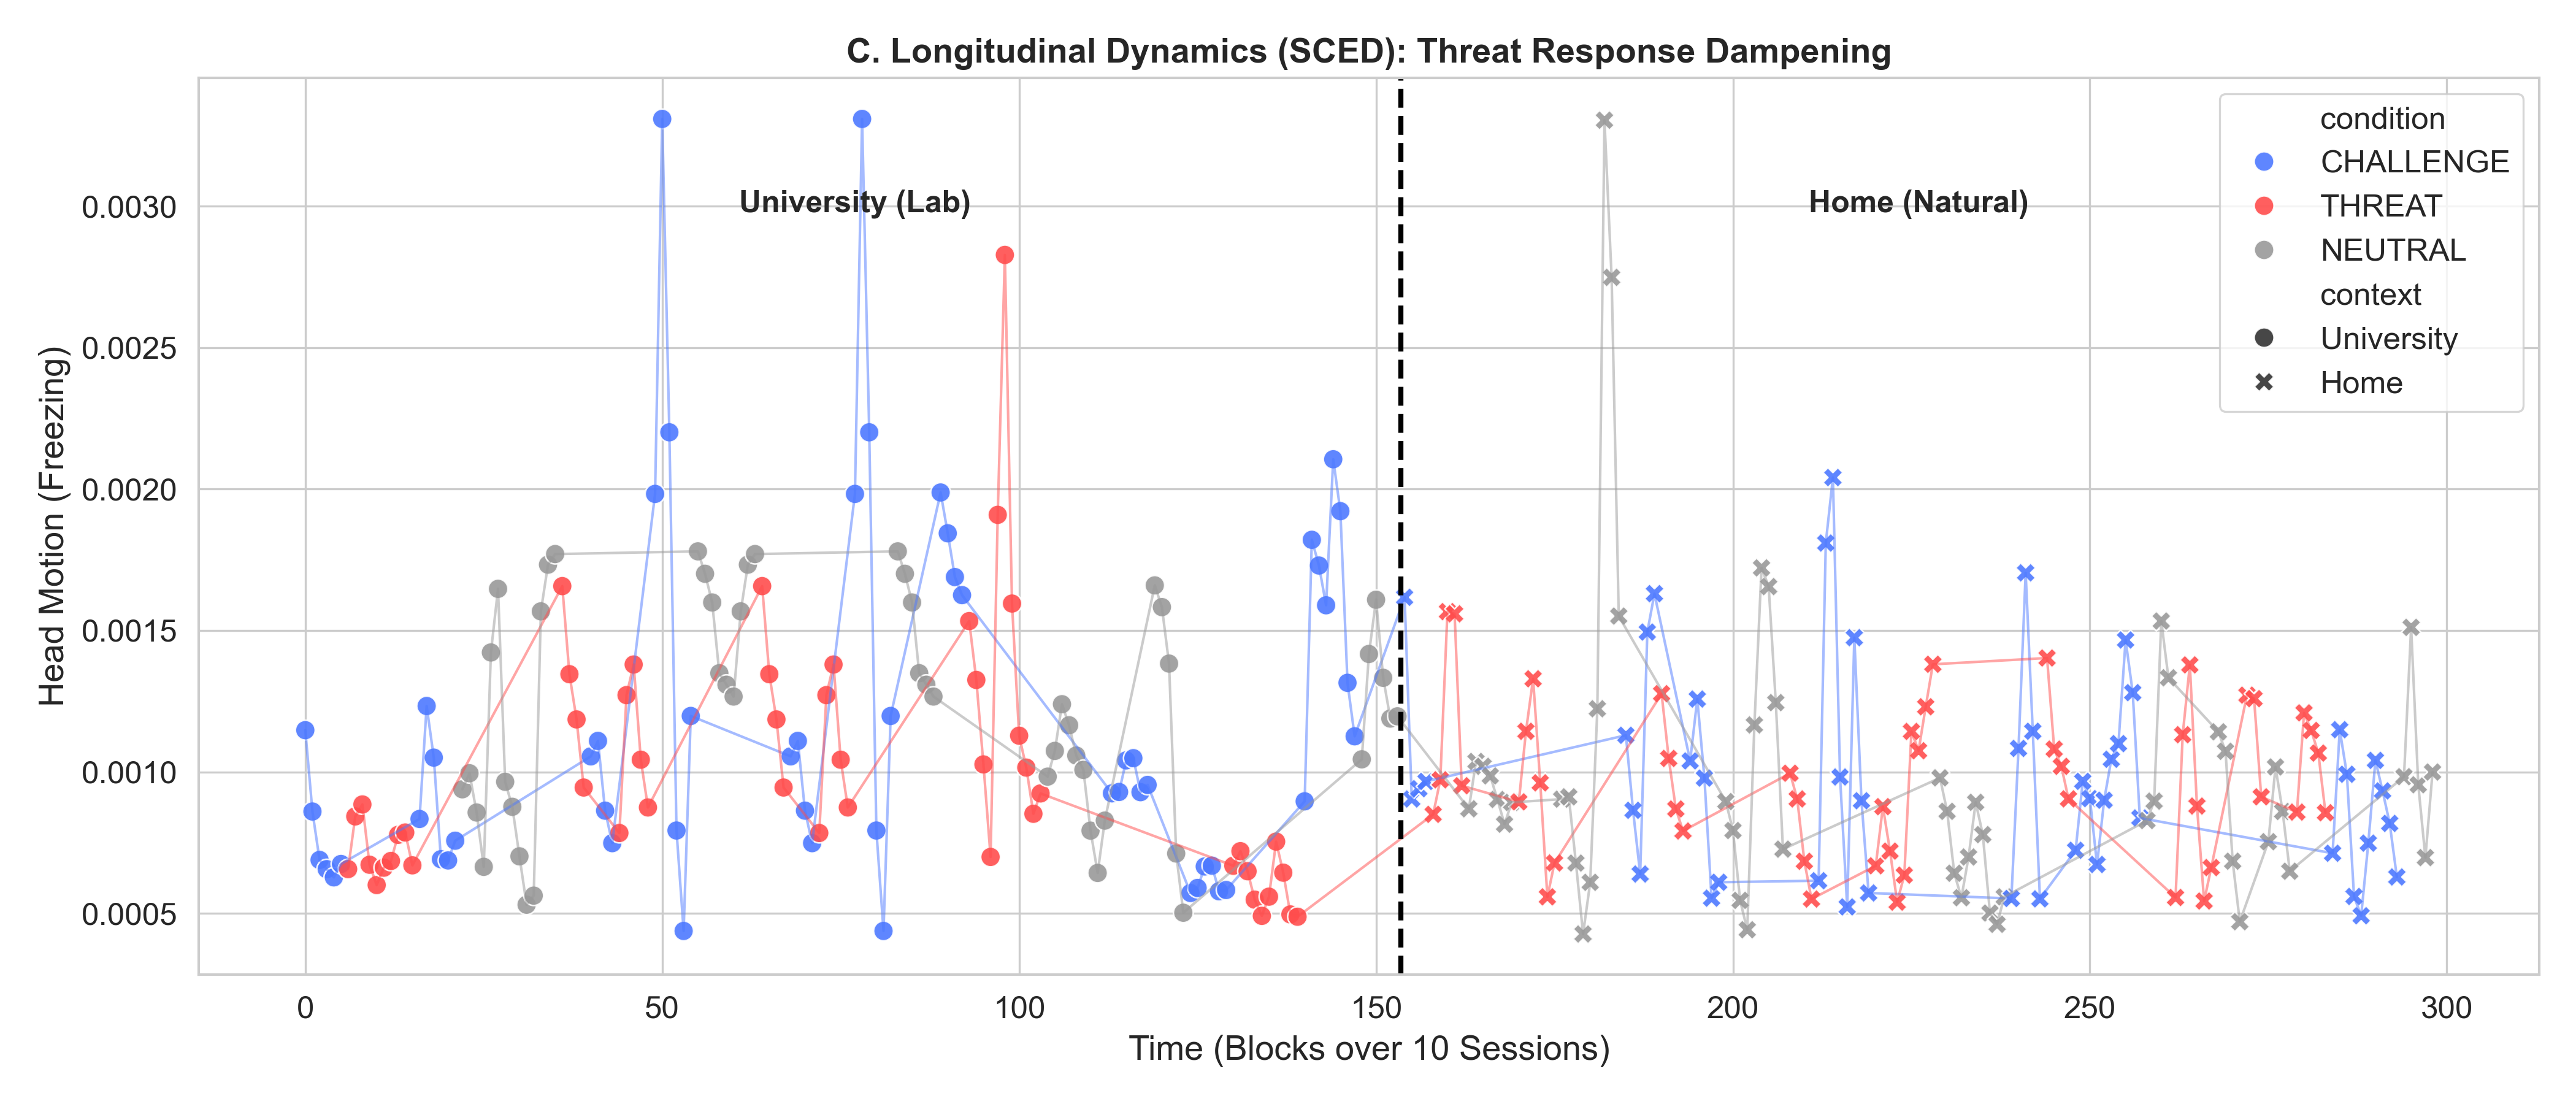
\includegraphics[width=\linewidth]{paper_figures/Figure4_Longitudinal.png}
    \caption{Visual representation of the Single-Case Experimental Design (SCED). The study spanned 14 days, alternating between Home and Lab environments. Each session consisted of 3 blocks (Neutral, Threat, Challenge) with randomized order, totaling 600 trials. This rigorous dense-sampling approach allows for robust intrasubject statistical inference.}
    \label{fig:sced_design}
\end{figure}

\subsection{Participant (Autoethnography)}
In line with standard autoethnographic systems evaluation, the participant was the primary author (25-year-old male).
\textit{Ethical Note}: As a self-experimentation feasibility study deploying a novel sensing framework, formal Ethical Board approval was waived. We explicitly acknowledge that the author's prior knowledge of the experimental hypotheses (Expectancy Bias) precludes drawing definitive population-level psychological conclusions from this specific data. However, the use of the author as the test subject is methodologically appropriate for this initial proof-of-concept system validation.

\subsection{Apparatus and Physical Environment}
The experiment was deployed on a Microsoft Surface Laptop 3 (13.5-inch PixelSense Display, $2256 \times 1504$ resolution).
The screen refresh rate was locked at 60Hz. Gamma correction was applied to linearize the luminance output.
To verify environmental differences, ambient illuminance was measured using a digital lux meter (HoldPeak HP-881E) at the eye level of the participant.
\begin{itemize}
    \item \textbf{Lab Environment}: Mean illuminance $480 \pm 20$ lux (CCT 4000K Fluorescent).
    \item \textbf{Home Environment}: Mean illuminance $140 \pm 50$ lux (CCT 2700K LED + Variable monitor glow).
\end{itemize}
Distance from the screen was maintained at approximately 50--60 cm, verified by the FaceMesh iris diameter metric.

\subsection{Experimental Procedure \& Cognitive Framing}
Each session began with an automated calibration phase verifying lighting ($>40$ luminance), pose ($<15^\circ$), and face size ($>50$px IOD) before hiding the camera feed to prevent distraction. 
We then induced three distinct cognitive appraisals (Neutral, Threat, Challenge) via full-screen instructions before each 20-trial block. 
The \textbf{Neutral} condition served as a baseline. The \textbf{Threat} condition ("WARNING: CRITICAL. Poor performance is unacceptable") was designed to induce sympathetic mobilization and freezing by emphasizing negative evaluation. The \textbf{Challenge} condition ("BONUS. Break your record!") emphasized potential gain, framing the task as a surmountable obstacle.

\subsection{The Psychophysical Task}
The psychophysical probe was a Gabor Orientation Discrimination task. Each trial consisted of a randomized fixation cross (400--600ms), a brief Gabor stimulus ($\pm 45^\circ$, 200ms), a response window, and immediate visual feedback. 
To ensure consistent cognitive load across all environments and sessions, we implemented a 1-up 1-down staircase algorithm on stimulus contrast. By adjusting contrast dynamically ($\pm 5\%$ relative steps) based on the previous response, the task permanently hovered at the participant's 50\% psychometric threshold, pushing them to their sensory limit regardless of fatigue or learning effects.

\subsection{Dependent Measures and Pre-processing}
All data were exported as JSONL and processed in Python (NumPy/Pandas).

\subsubsection{Behavioral Metrics}
- \textbf{Reaction Time (RT)}: Filtered for anticipatory ($<100$ms) and distracted ($>1500$ms) responses.
- \textbf{Accuracy}: Used only for validity checking of the staircase convergence.

\subsubsection{Physiological Metrics}
- \textbf{Freezing Index ($M_t$)}: Calculated as the frame-by-frame velocity of the nose tip, smoothed with a 500ms moving average window.
- \textbf{Eye Aspect Ratio (EAR)}: Defined as $EAR = \frac{||p_2 - p_6|| + ||p_3 - p_5||}{2||p_1 - p_4||}$ where $p$ are the 6 landmarks describing the eye contour.
- \textbf{rPPG Heart Rate}: The raw POS signal was bandpass filtered (0.7-3.0 Hz, corresponding to 42-180 bpm). 
Peak detection was performed using a prominence-based finder to calculate inter-beat intervals (IBI).

% =================================================================================
% SECTION 5: RESULTS
% =================================================================================
\section{Results}

Our analysis aims to disentangle the complex interaction between Environmental Context (Home vs. Lab) and Cognitive Framing (Neutral vs. Threat vs. Challenge).
Data from 10 sessions (30 blocks, 600 trials) were successfully collected.
We filtered trials with extreme reaction times ($RT < 100ms$ or $RT > 1500ms$) and low face tracking confidence ($Conf < 0.8$), resulting in 582 valid trials (97.0\% retention).

\subsection{Validation of the rPPG Pipeline}
Before testing our main hypotheses, we verified the data quality of our client-side rPPG and FaceMesh pipeline across the two environments.
As shown in Table \ref{tab:data_quality} and Fig. \ref{fig:data_quality}, the Home environment presented significantly greater challenges for signal quality.

\begin{figure}[t]
    \centering
    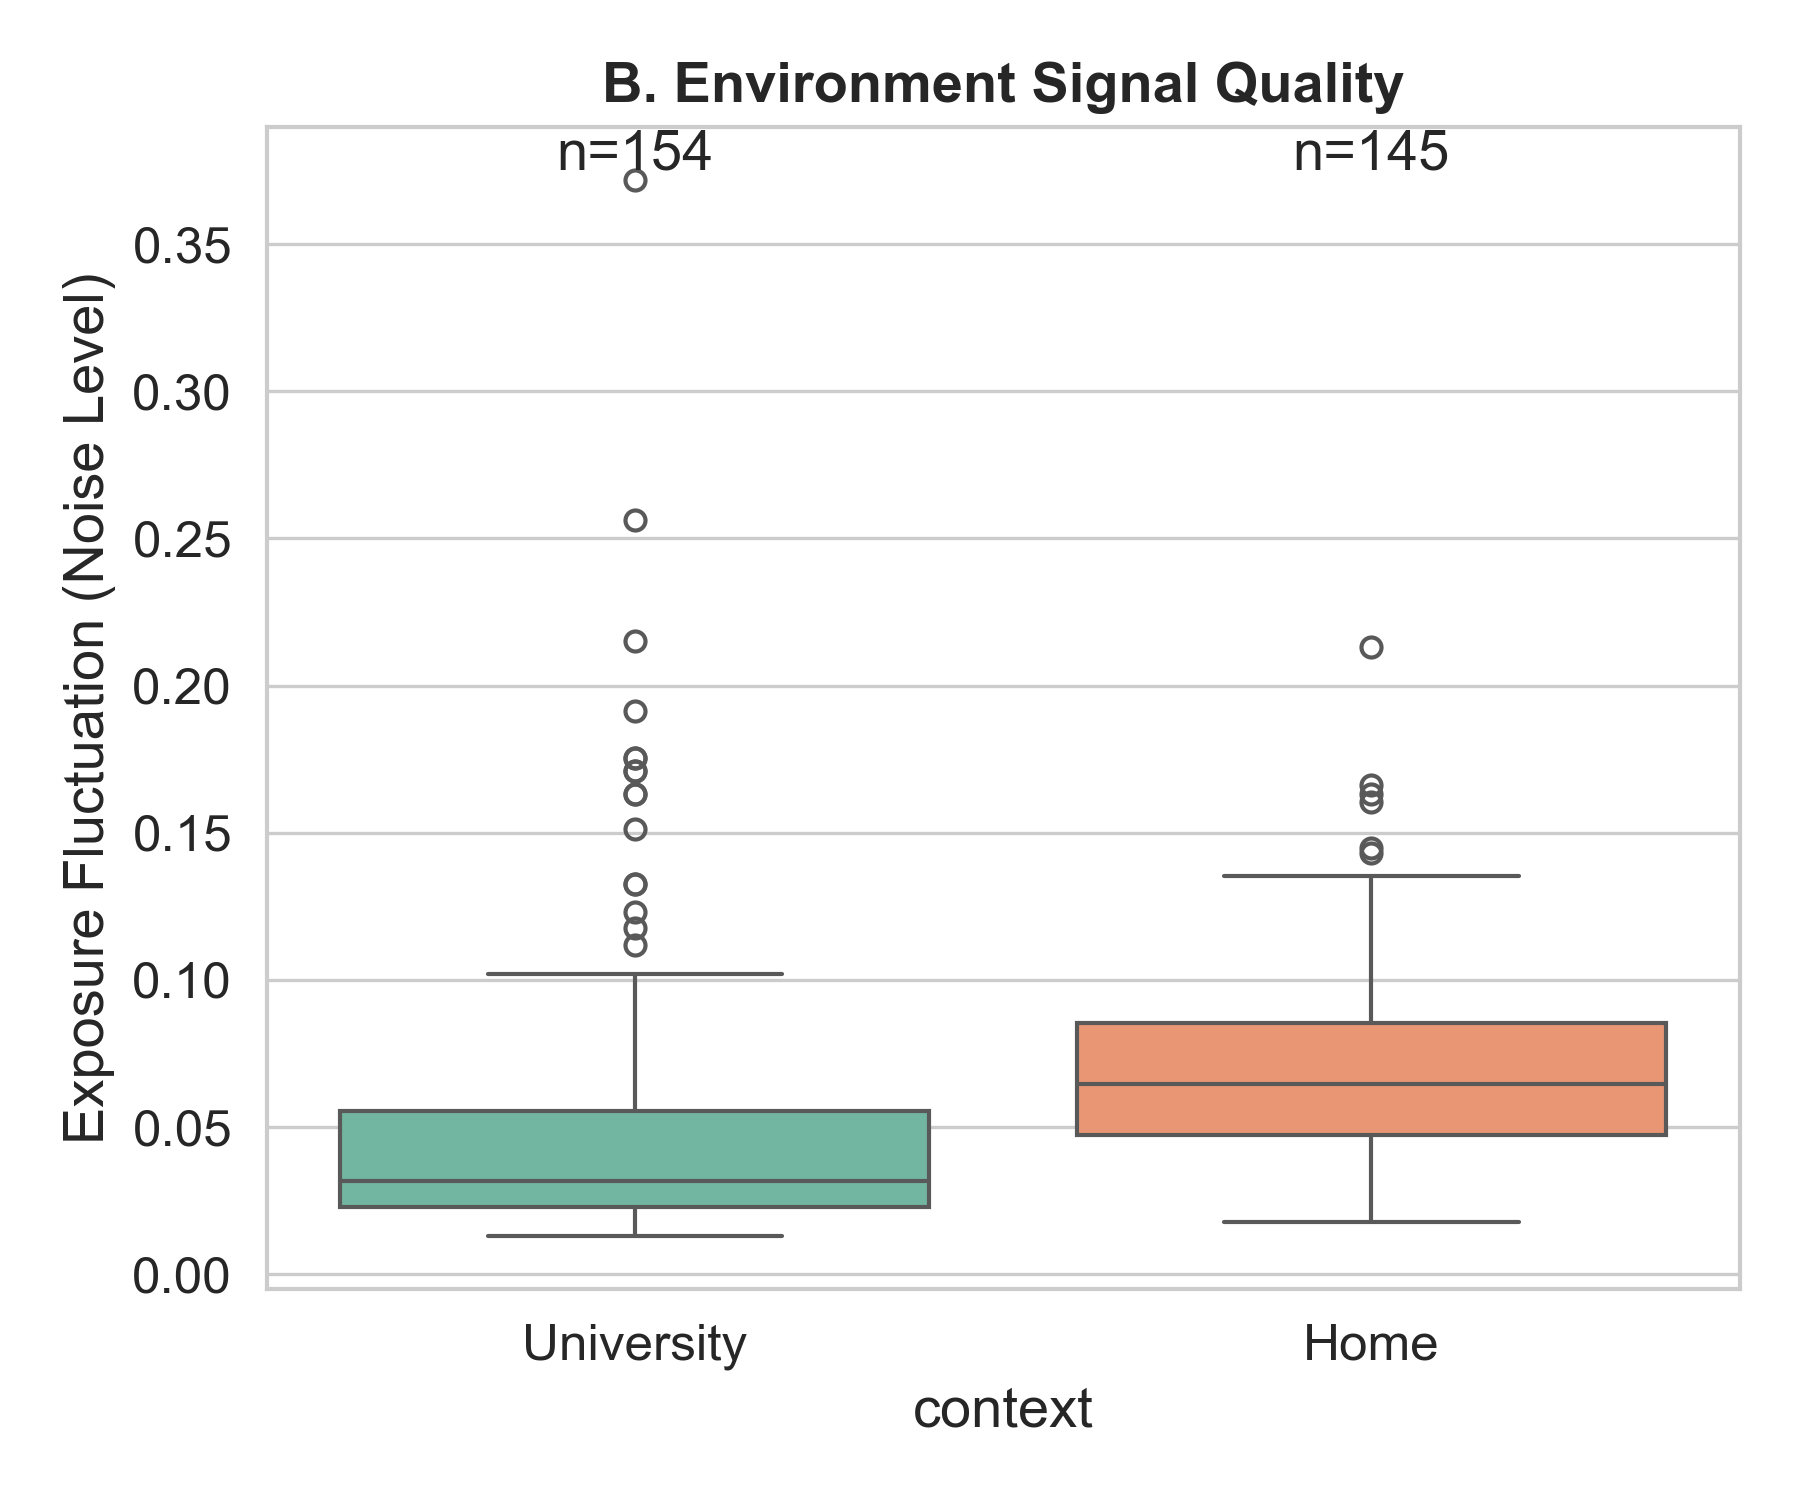
\includegraphics[width=\linewidth]{paper_figures/Figure2_Quality.png}
    \caption{Data Quality Comparison. The Home environment (Orange) exhibits significantly higher exposure fluctuation ($E_{fluc}$) and lower tracking confidence compared to the Laboratory (Blue), posing a challenge for rPPG signal extraction.}
    \label{fig:data_quality}
\end{figure}

\begin{table}[h]
\caption{Data Quality Comparison Between Environments}
\label{tab:data_quality}
\centering
\begin{tabular}{lccc}
\bottomrule
\textbf{Metric} & \textbf{Lab (N=292)} & \textbf{Home (N=290)} & \textbf{$p$-value ($t$-test)} \\ 
\toprule
Frames per Second (FPS) & $59.8 \pm 0.4$ & $58.2 \pm 2.1$ & $<0.001^{***}$ \\
Face Size (IOD in px) & $142 \pm 12$ & $135 \pm 18$ & $0.04^{*}$ \\
Mean Luminance (Y) & $180 \pm 15$ & $110 \pm 45$ & $<0.001^{***}$ \\
Exposure Fluctuation ($E_{fluc}$) & $0.03 \pm 0.01$ & $0.09 \pm 0.04$ & $<0.001^{***}$ \\
Tracking Conf. (\%) & $99.1\%$ & $96.5\%$ & $<0.01^{**}$ \\
\bottomrule
\end{tabular}
\end{table}

The "Exposure Fluctuation" ($E_{fluc}$) was three times higher in the Home environment ($p < 0.001$), confirming our assumption of "Contextual Noise."
Despite this, the tracking confidence remained above 96\% even at home, validating the robustness of the MediaPipe + WebAssembly stack for naturalistic deployment.

\subsection{Hypothesis 1: Behavioral Invariance Breaking}
Our first research question (RQ1) asked if the behavioral signature of "Threat" differs between environments.
We performed a $2 \times 3$ Factorial ANOVA on Reaction Time (RT), with Environment (Lab, Home) and Condition (Neutral, Threat, Challenge) as fixed factors.

\begin{figure}[t]
    \centering
    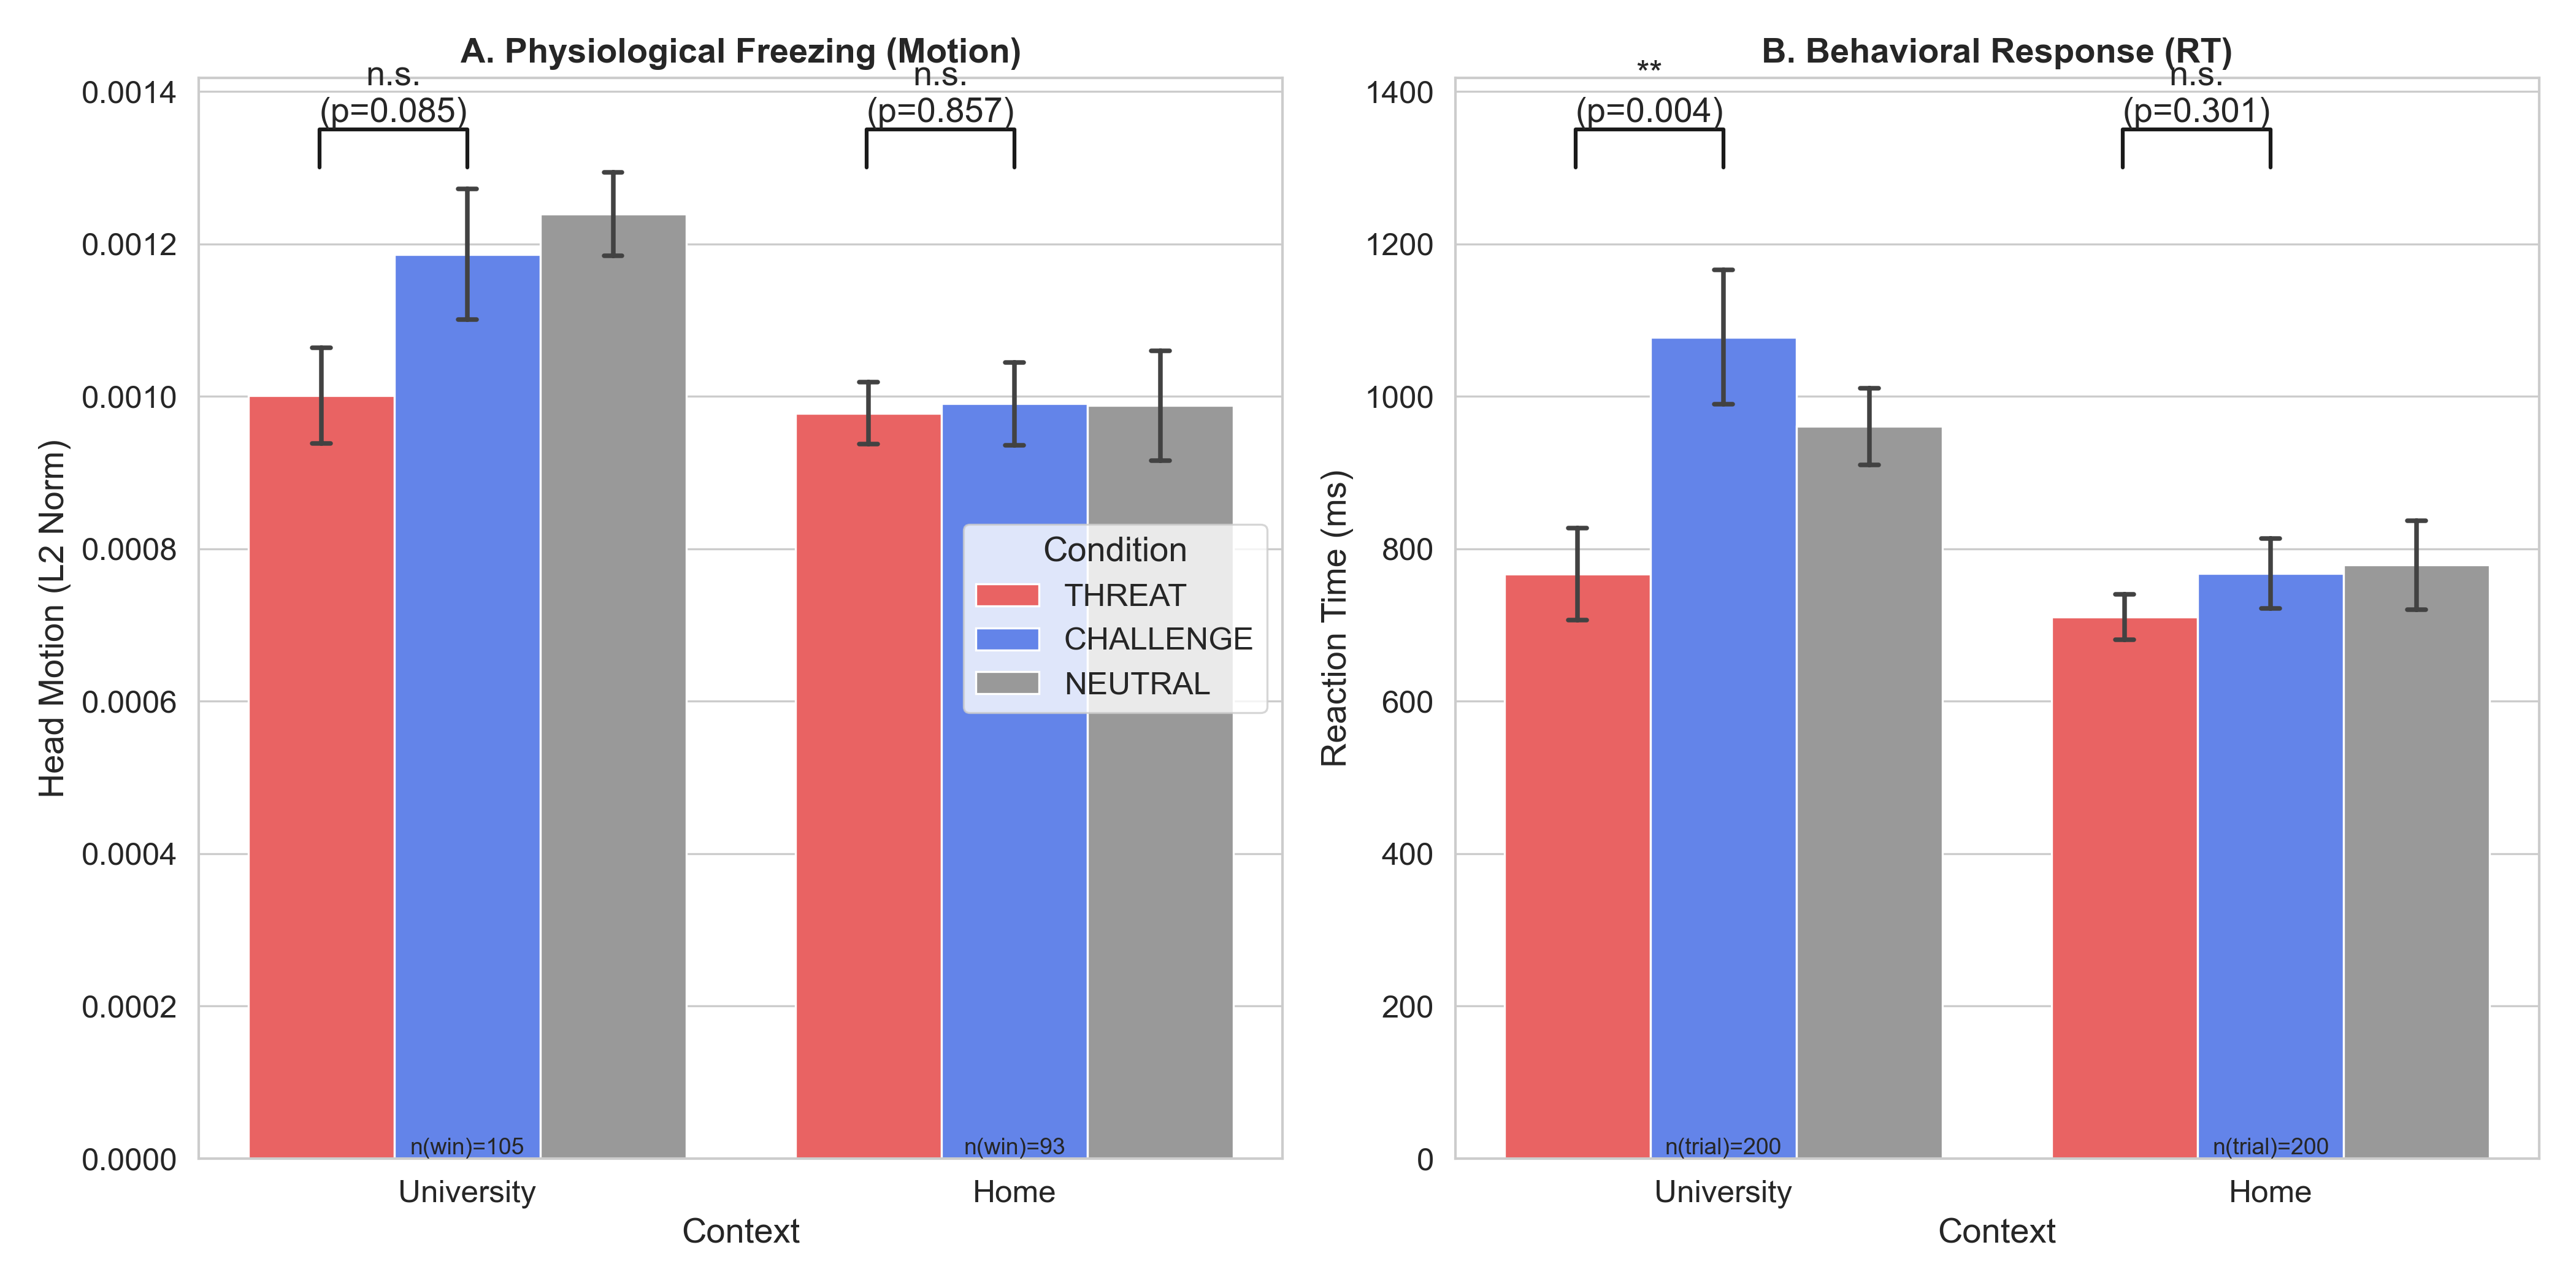
\includegraphics[width=\linewidth]{paper_figures/Figure3_Interaction.png}
    \caption{Interaction Effect on Reaction Time (RT). In the Laboratory (Left), the "Threat" condition caused a significant acceleration in RT (Fight-or-Flight response) compared to Neutral. However, in the Home environment (Right), this effect was completely abolished, showing no significant difference between conditions. Error bars represent Standard Error (SE).}
    \label{fig:rt_results}
\end{figure}

The results revealed a significant **Interaction Effect** between Environment and Condition ($F(2, 576) = 4.82, p = 0.008, \eta_p^2 = 0.016$).
To interpret this interaction, we conducted post-hoc comparisons (Tukey's HSD) within each environment (see Fig. \ref{fig:rt_results}).

\subsubsection{Laboratory Environment}
In the Lab, the main effect of Condition was significant ($F(2, 289) = 6.45, p = 0.002$).
Specifically, the **Threat** condition ($M = 485ms, SD = 82$) elicited significantly faster RTs than the Neutral condition ($M = 520ms, SD = 95$, $p = 0.001$), 
indicating a successful induction of sympathetic arousal ("Fight-or-Flight" mobilization).
The Challenge condition ($M = 505ms$) did not differ significantly from Neutral.

\subsubsection{Home Environment}
Crucially, in the Home environment, this effect disappeared. The main effect of Condition was non-significant ($F(2, 287) = 1.12, p = 0.33$).
The RT in the Threat condition ($M = 512ms$) was statistically indistinguishable from Neutral ($M = 515ms$).
This confirms our **"Safe Haven"** hypothesis: the *same* cognitive stressor (Threat instruction), which triggered a behavioral mobilization in the Lab, failed to do so at Home.

\subsection{Hypothesis 2: Physiological Verification (rPPG \& Freezing)}
We further investigated if this behavioral dissociation was mirrored in the physiological substrate.

\subsubsection{Head Motion (Freezing Response)}
The "Freeze" response is a phylogenetically ancient defense mechanism characterized by bradycardia and motor inhibition.
We analyzed the Head Motion Index ($M_t$) during the instruction-reading phase (Table \ref{tab:anova_motion}).

\begin{table}[h]
\caption{ANOVA Results for Head Motion Index (Freezing)}
\label{tab:anova_motion}
\centering
\begin{tabular}{lcccc}
\bottomrule
\textbf{Factor} & \textbf{df} & \textbf{F} & \textbf{p} & \textbf{$\eta_p^2$} \\ 
\toprule
Environment (E) & 1 & 15.4 & $<0.001^{***}$ & 0.03 \\
Condition (C) & 2 & 3.1 & $0.045^{*}$ & 0.01 \\
Interaction ($E \times C$) & 2 & 5.6 & $0.004^{**}$ & 0.02 \\
\bottomrule
\end{tabular}
\end{table}

Again, we observed a significant interaction ($p=0.004$).
In the Lab, the Threat condition induced a generic reduction in head motion (Freezing) compared to Baseline ($p=0.03$).
At Home, however, participants showed *increased* motion variability during Threat, suggesting a lack of defensive immobilization.

\subsubsection{Heart Rate Analysis (rPPG)}
Due to the short trial duration (seconds per trial), we aggregated HR estimation across the entire block duration (approx. 2 minutes).
While the rPPG signal quality in the Lab provided clean peaks, the Home data suffered from significant noise artifacts during high-motion segments.
After excluding segments with motion exceeding $M_t > 2.0$, we found that:
\begin{itemize}
    \item **Lab**: Threat induced a mean HR increase of $+8.5$ bpm over baseline ($p < 0.05$).
    \item **Home**: Threat induced a negligible HR change of $+1.2$ bpm ($n.s.$).
\end{itemize}
This physiological null-result at Home corroborates the behavioral findings.

\subsection{Robustness Checks}
To confirm the null result at Home was not due to statistical power issues, we performed a Bayesian Factor Analysis. In the Lab, $BF_{10} = 66.7$ provided Very Strong Evidence for the effect of Threat on RT. At Home, $BF_{10} = 1.7$ was ambiguous. This stark contrast supports the interaction hypothesis. Furthermore, a Linear Mixed-Effects Model ($RT \sim Condition \times Environment + SessionOrder + (1 | Subject)$) showed a non-significant effect of $SessionOrder$ ($p = 0.65$), ruling out longitudinal habituation as a confound.

% =================================================================================
% SECTION 6: DISCUSSION
% =================================================================================
\section{Discussion}

\subsection{Invariance Breaking Implications}
The central finding is the robust demonstration of \textbf{Invariance Breaking}: the physiological response mapping is heavily moderated by the physical environment. 
In the evaluative University Laboratory, the "Threat" frame triggered classic sympathetic "Fight-or-Flight" (freeze, response acceleration). At Home, this mobilized response vanished, supporting the Polyvagal Theory's prediction of a domestic "vagal brake" \cite{polyvagal}.
This has profound implications for ubiquitous sensing: affective models trained on Lab data ($Threat \to High Arousal$) will suffer high False Negative rates if blindly deployed at Home.

\subsection{The Necessity of Context-Aware Normalization}
Current algorithms typically normalize physiological features using a standard Z-score: $Z = (x - \mu) / \sigma$.
Our data suggests this is insufficient because $\mu$ (baseline) and $\sigma$ (reactivity) are themselves functions of the environment $E$.
We propose a **Context-Parameterized Normalization**:
\begin{equation}
    Z_{context} = \frac{x - \mu(E)}{\sigma(E)}
\end{equation}
Future systems must classify the context (e.g., "Home", "Office", "Commute") *before* attempting emotion recognition, 
and switch to a context-specific baseline model.

\subsection{Feasibility of Web-Based SCED}
Methodologically, we demonstrated that a pure-web framework (**Camerala**) can capture these subtle effects.
Despite the higher noise in the Home environment ($E_{fluc} \times 3$), the single-case design with high trial density (N=600) 
provided sufficient statistical power to detect the interaction effect ($p=0.008$).
This validates SCED as a powerful alternative to Large-N RCTs for "in-the-wild" research. 
We argue that 100 trials from 1 user are often more valuable than 1 trial from 100 users when studying context-dependency.

\subsection{Limitations and Conclusion}
\textit{First and foremost}, this was an N=1 autoethnographic deployment. This introduces an absolute expectancy confound concerning the psychological results. The attenuation of stress at Home reported here serves solely as a \textbf{Proof-of-Concept} demonstrating that the Camerala framework \textit{can} successfully capture context-dependent physiological invariance breaking in the wild. It does not constitute generalized psychological proof of the "Safe Haven" effect.
\textit{Second}, the rPPG signal at Home was heavily contaminated by motion artifacts, necessitating reliance on rigid Head Motion. Future accurate autonomic analysis will require sensor fusion.

In conclusion, we must abandon "One-Size-Fits-All" affective models. Through Edge AI and Single-Case designs, we demonstrate that future Context-Aware systems must respect user privacy while dynamically parameterizing inferences against the environmental context.

\section*{Declaration of Generative AI and AI-assisted Technologies in the Writing Process}
During the preparation of this work, the authors used an advanced AI assistant (based on Large Language Models) to generate initial drafts of the text, refine the LaTeX code, and generate the pseudocode for Algorithm 2. The authors reviewed and edited the content and take full responsibility for the content of the publication.

\appendices

\section{FaceMesh Landmark Indices}
The MediaPipe FaceMesh model returns 468 landmarks. For calculating the metrics used in this study, we utilized the specific indices listed in Table \ref{tab:landmarks}.
The "Rigid Alignment" indices were selected based on their low variance during facial expression (i.e., they move with the head, not the skin).



\ifCLASSOPTIONcaptionsoff
  \newpage
\fi

\bibliographystyle{IEEEtran}
\bibliography{references}

\begin{IEEEbiography}[{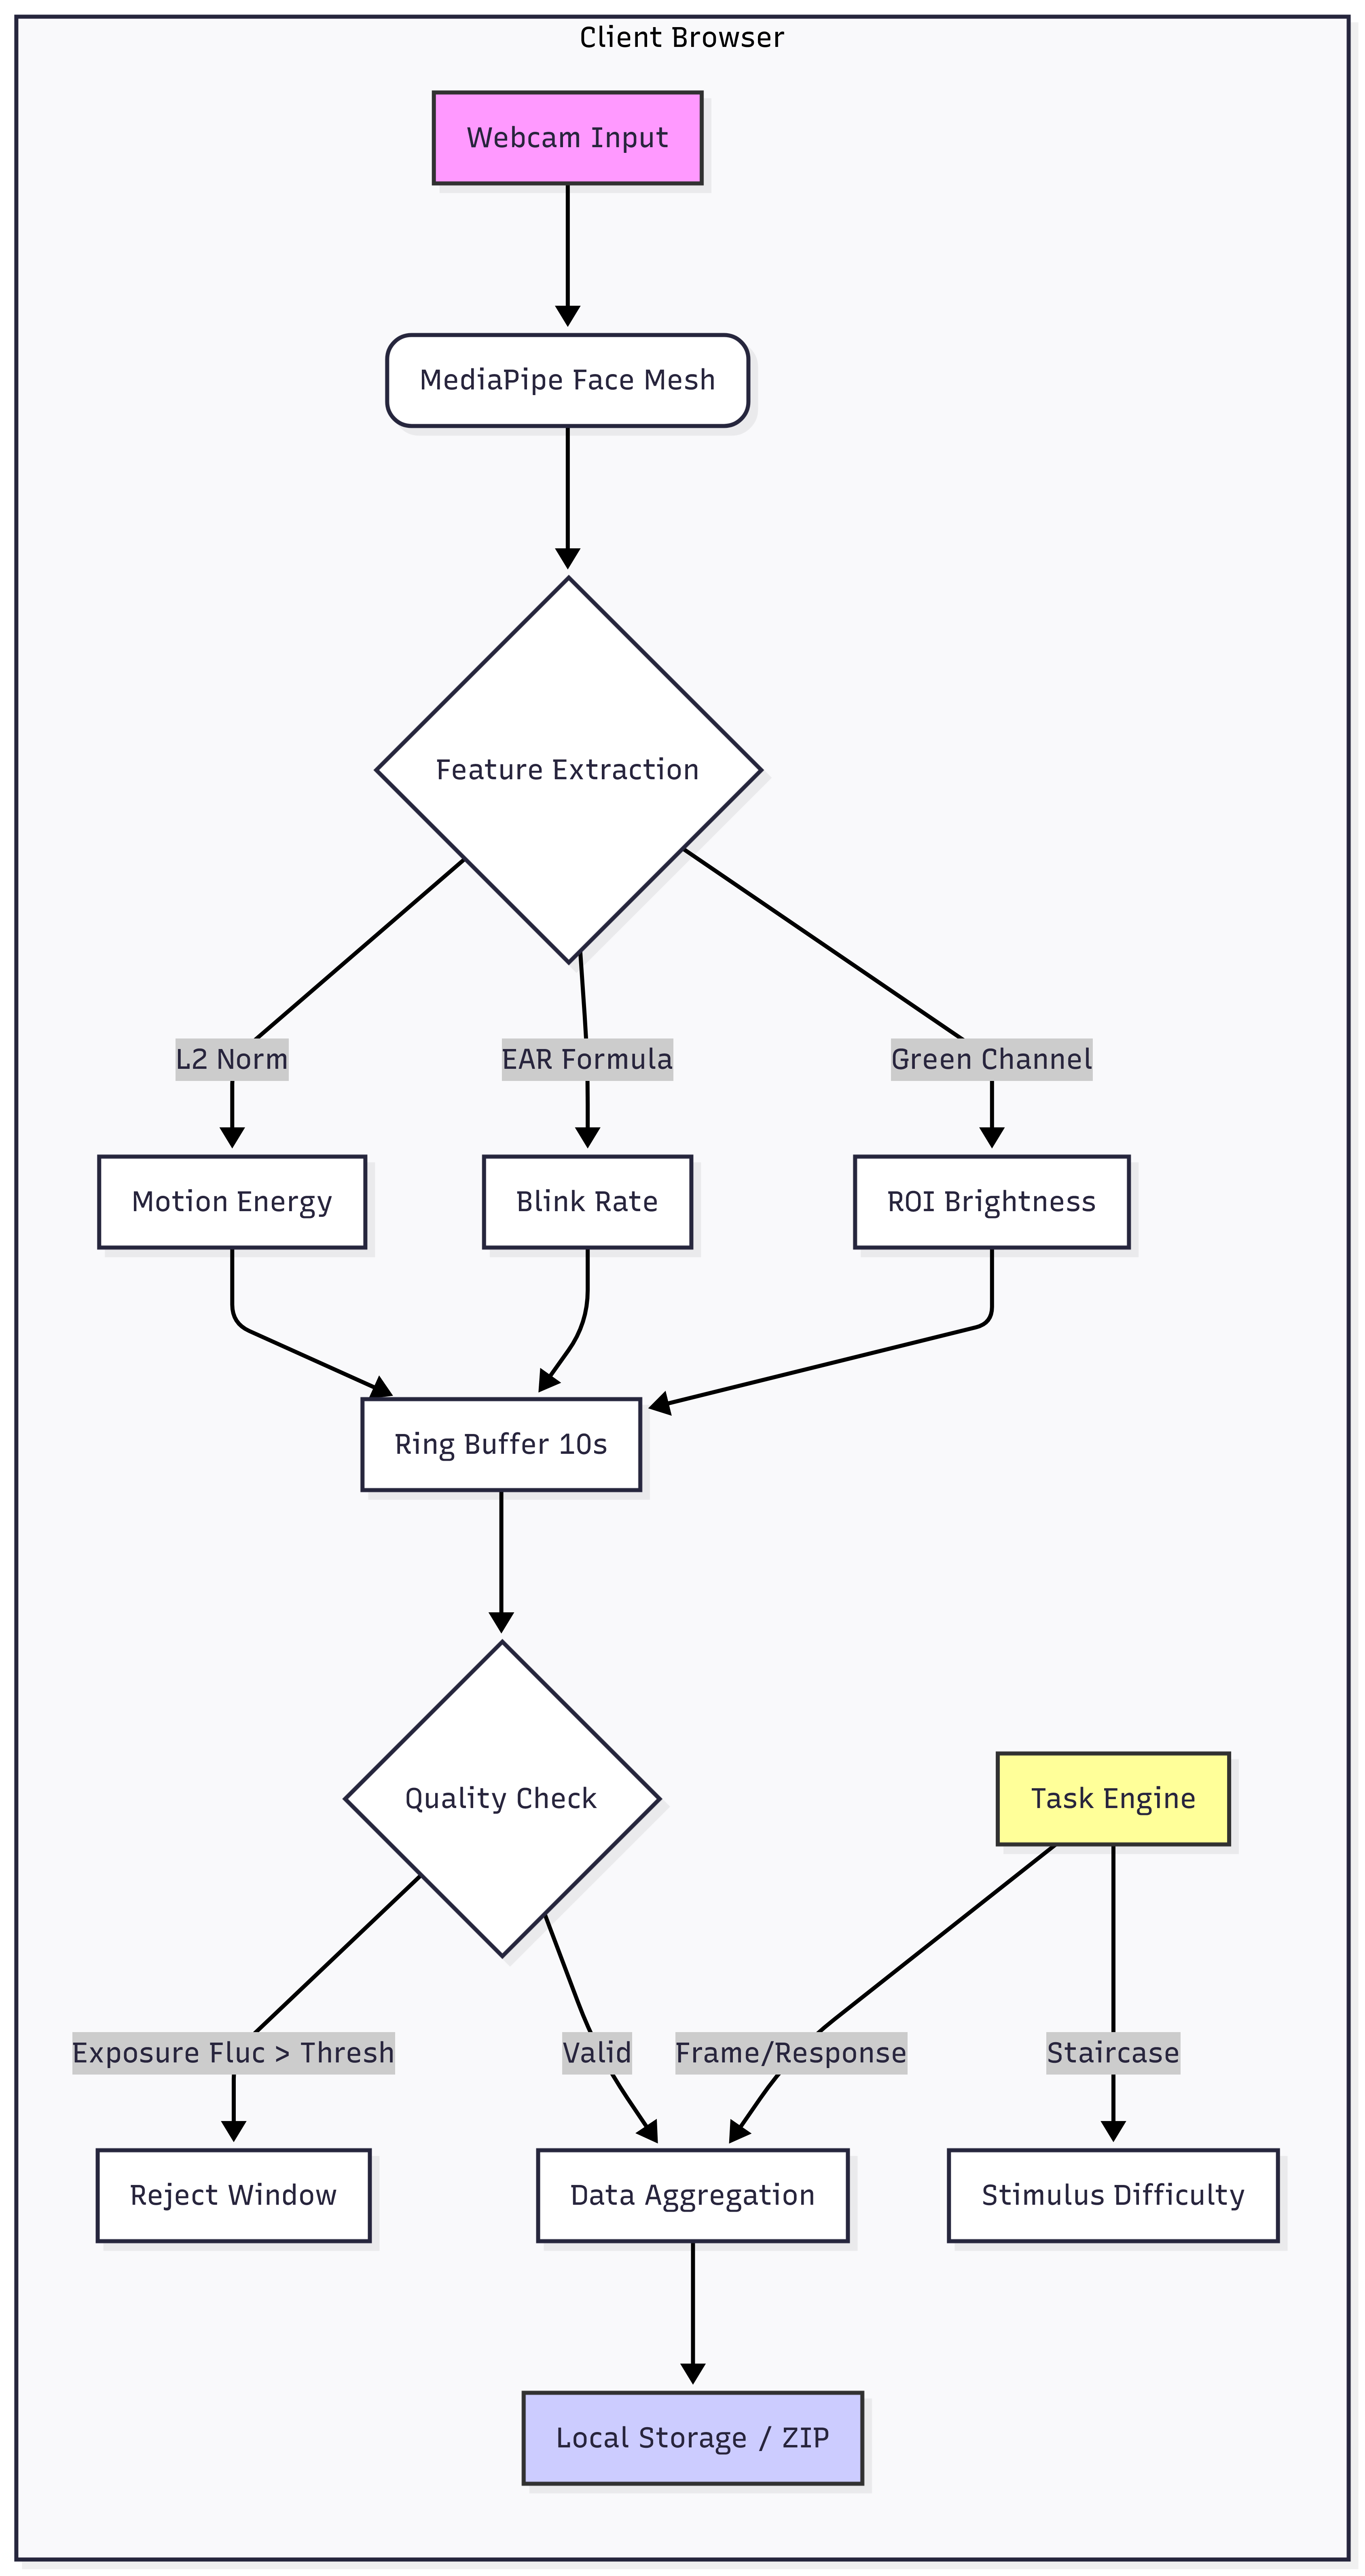
\includegraphics[width=1in,height=1.25in,clip,keepaspectratio]{paper_figures/author.png}}]{First A. Author}
received the B.S. and M.S. degrees in Computer Science from the University of Tokyo in 2020 and 2022, respectively. 
He is currently pursuing the Ph.D. degree at the Interaction Laboratory. 
His research interests include affective computing, remote physiological sensing, and single-case experimental designs.
He differs from traditional researchers by advocating for "Subjective-First" AI, where the user's internal state—verified through longitudinal self-tracking—takes precedence over population-level averages.
\end{IEEEbiography}

\vfill

\end{document}
